\section{Constructing Examples in \datasetnameemoji~At Scale}
\label{sec:curation}
We develop a modular data curation pipeline—powered by GPT-4o~\citep{hurst2024gpt}—to synthesize persona-oriented, multi-session user–model conversations with long context. The pipeline minimizes irrelevant or randomly injected content to better evaluate how effectively LLM chatbots address the challenges outlined in Section~\ref{sec:overview}, while ensuring cost-effectiveness and scalability: generating data for each persona on each conversation topic costs approximately \$2, independent of the context window length up to 1$M$ tokens.


% We develop a modular data curation pipeline—powered by GPT-4o~\citep{hurst2024gpt}—to synthesize high-quality, persona-oriented, and multi-session user–model conversations with long context, minimizing irrelevant or randomly injected context, in order to evaluate how well language models address the challenges outlined in Section~\ref{sec:overview}, while maintaining cost-effectiveness and scalability.

% \datasetname~ features synthetic multi-session user-chatbot interactions centered around user personas, minimizing irrelevant or randomly injected context


% Given a conversational session and its associated meta-data of events and facts, we then generate grounded questions.




% \begin{figure}[t]
%   \centering
%   \includegraphics[width=1\linewidth]{figures/concatenate.pdf}
%   \caption{TODO}
%   % \vspace{-3mm}
%   \label{fig:concatenate}
% \end{figure}



% To evaluate the language model's performance on tasks requiring persona-aligned information from long-memory conversation datasets, we introduce a high-quality, diverse, and scalable data curation pipeline. Our approach replicates real-world scenarios in which LLM agents must retain user memory and adapt to diverse personas and unique interaction histories. Unlike benchmarks that focus solely on simple facts presented in short paragraphs or on lengthy yet contexts lacking relevance, \datasetname\ ensures that every interaction is anchored to a specific user persona engaging with the agent on a defined topic while maintaining temporal coherence. The following sections detail our systematic and scalable approach to curate long conversational data.

% In this section, we introduce our data curation pipeline to curate high-quality, multi-turn, and multi-session conversational data, in order to evaluate how well langauge models can adddress the challenges discussed in Section~\ref{sec:overview}. 
% Unlike existing memory benchmarks that either focus solely on the accuracy of simple facts or adopt a needle-in-a-haystack approach by injecting key phrases into loosely connected long contexts, \datasetname\ ensures that every interaction is anchored to a specific user persona engaging with the model on a specific topic, while maintaining temporal coherence. TODO: We can talk about this in intro or related work

% Generating high-quality long-form conversational data from scratch remains challenging, 
% % especially if one wants to generate millions of tokens from scratch.
% To address this, we introduce a modularized data curation pipeline that first focuses on generating individual conversation sessions and concatenates them afterwards to a satisfactory length, enabling cost-effective and scalable long-context generation.

% designed to generate high-quality, multi-turn, and multi-session conversational data
% replicating real-world scenarios in which language models must retain memory of the users and adapt to diverse user personas.

\paragraph{Constructe user profile and persona.}
We sample a set of random personas from \personahub~\citep{ge2024scaling}, each comprising about one to three sentences, and augment them with additional demographic information and extended personal details. We also construct a timeline and populate it with events that align with the persona. These events serve as the \textit{general personal history}, such as education, career development, and life experiences, to provide a richer context. The prompts used in the process can be found in Appendix~\ref{app:prompts}.


% We begin by collecting a diverse set of user personas from \personahub~\citep{ge2024scaling} that offers a billion synthetic personas, each consisting of approximately one to three sentences. We then expand these personas with additional details, including age, racial and gender identities, occupations, educational backgrounds, and other relevant characteristics. We further prompt OpenAI's GPT-4o model to propose five hobbies this person likes and dislikes, respectively, as the initial user preferences.


% \subsection{Generate Topic-Specific Personal Histories}
Building on the persona and general personal history, we generate one additional \textit{topic-specific personal history} for each conversation topic. Under each topic, we define a set of initial preferences, ensuring no overlap across different topics. Each topic-specific history includes events, timestamps, associated preferences, potential updates to those preferences, and the underlying reasons for those changes. This approach ensures a coherent progression of user experiences while maintaining a strong connection to their personas.


The structured personal histories also facilitate the curation of question–answer pairs. We leverage short-form information within these histories to extract ground-truth user profiles and preferences at any specific time, ensuring that the correct answers are both event- and persona-grounded. In contrast, distractor options, while generally reasonable, either overlook the user’s persona or contradict it. Additionally, we exclude all questions that the model can answer correctly without seeing any contextual information from the benchmark.



% We prompt GPT-4o to expand the initial persona into two chronological personal histories: general and topic-specific. The general history captures broad life events like college graduation related to the persona, which will be shared across all conversation topics. Each conversation topic will have its own topic-specific personal history.

% % Along the temporal axis of each personal history, 
% We generate $10$ events within last 10 years this user might have experienced, including both short-term and long-term ones. Each event is timestamped and linked to one of the five likes or dislikes defined in the persona.
% We further extend this process to generate personal histories for three other time periods: from now to next week, next week to next month, and next month to next year. Each period may introduce events linked to new likes or dislikes mentioned in the persona, as well as events with preference changes from the previous period accompanied by detailed reasons for the change. This approach ensures a coherent progression of user experiences while maintaining a strong connection to their preferences. 

\paragraph{Simulate conversation sessions from user profile.}
We divide the timeline into multiple segments, resulting in segments of personal histories that follow a causal, chronological order. Each segment is then expanded into a full user–model conversation session, designed to cover all details of the corresponding topic-specific personal history segment, together with additional storytelling context as if the user is talking with a chatbot naturally. For example, under the therapy consultation topic, we frame the interaction as a user seeking guidance from an AI therapist. 

To enhance the quality of the conversations, we incorporate several tricks: (1) Before generating each user–model interaction turn, we prompt GPT-4o to first identify and cite the relevant event from the personal history. These citations serve as internal guidance and are not included in the final evaluation data. (2) Since GPT-4o may miss some events, leading to incomplete preference update sequences, we employ a self-reflection mechanism. We ask GPT-4o to review the generated conversation and identify any missing events from the personal history, ensuring better coverage and coherence across the interaction.

% During evaluation, the model will only have access to conversations, not personal histories.

% Writing and coding topics are not tied to personal histories. Instead, we prompt GPT-4o to infer each user's explicit style and formatting preferences from their persona, avoiding subjective ones. Using real-world samples, we query GPT-4o to rewrite each sample to reflect these personalized preferences. We then simulate a user interacting with an AI writing or coding assistant to convert each original sample to the persona-aligned one. In these dialogues, the user highlights specific sentences or code pieces they find unsatisfactory in terms of style or format, and the assistant offers targeted editing suggestions.


% Once we have detailed personal histories, we have the foundation for generating actual conversations. Under each topic, we generate four causally connected conversation sessions, spanning from \textit{about 10 years ago to the present, from now to next week, from next week to next month, and from next month to next year.} Specifically, we prompt GPT-4o to transform each detailed history into a multi-turn conversation under the current topic. For example, when simulating a therapy consultation, we frame the interaction as a user seeking guidance from an AI therapist, trying to discuss every single event from their general and therapy-specific history. When generating each utterance, we ask GPT-4o to first cite relevant personal histories, including the timestamps, as side notes. Note that during evaluation, these side notes will be hidden from the model being assessed. 
% using a single thread in the OpenAI's Assistant API for each topic.

% However, two potential issues remain: (1) the conversation that GPT-4o generated may not cover all events in the personal histories. This is crucial because, \textit{during evaluation, models will have access only to the conversations, not the personal histories.} These histories are solely used for curating conversation data and evaluation questions. As a result, if certain events are missing from the conversations, the model will have no way to answer questions curated from these events. (2) We still find that each conversation may not be long enough.
% \begin{itemize}
%     \item We mitigate the first issue by leveraging \textit{self-reflection}. By providing the model with the target personal histories with all timestamps, along with the generated conversation with side notes, we prompt it to self-check for any missing timestamps and if any, insert them by generating new utterances. We find this helps cover the majority of previously missing events.
%     \item We address the second issue by prompting GPT-4o-mini to expand each pair of user and model utterances to at least five sentences, adding irrelevant context and details without alterning original meaning or user preferneces. This approach extends the final conversation length by approximately five times.
    % \item We address the second issue by breaking the conversation into utterance groups, each consisting of a side note, the user's utterance, and the model's response for a single event—typically totaling three sentences. We send each utterance group to GPT-4o-mini, requesting it to expand each utterance to at least five sentences by adding irrelevant context and details while preserving the original meaning. This approach helps expand the final conversation length by approximately five times.
% \end{itemize}


% \subsection{Curating Conversation Data for Writing Topics with Special Steps}
% Writing topics are not based on personal histories; instead, we query GPT-4o to propose the user's explicit style and format preferences based on personas. Using real-world writing samples in creative writing, email composition, and code programming, we prompt GPT-4o again to rewrite each sample to align with the user's specific style and format preferences. Next, given both a general and a persona-aligned sample, we transform them into multi-turn conversations, simulating a scenario where the user consults an AI writing assistant to refine their original work. In these conversations, the user explicitly refers to a sentence from the original sample, complaining about style or format issues, and the assistant provides editing suggestions. Different from other topics, these topics consist of multiple independent sessions, each generated from separate original writing or coding samples.
\begin{figure}[t]
  \centering
  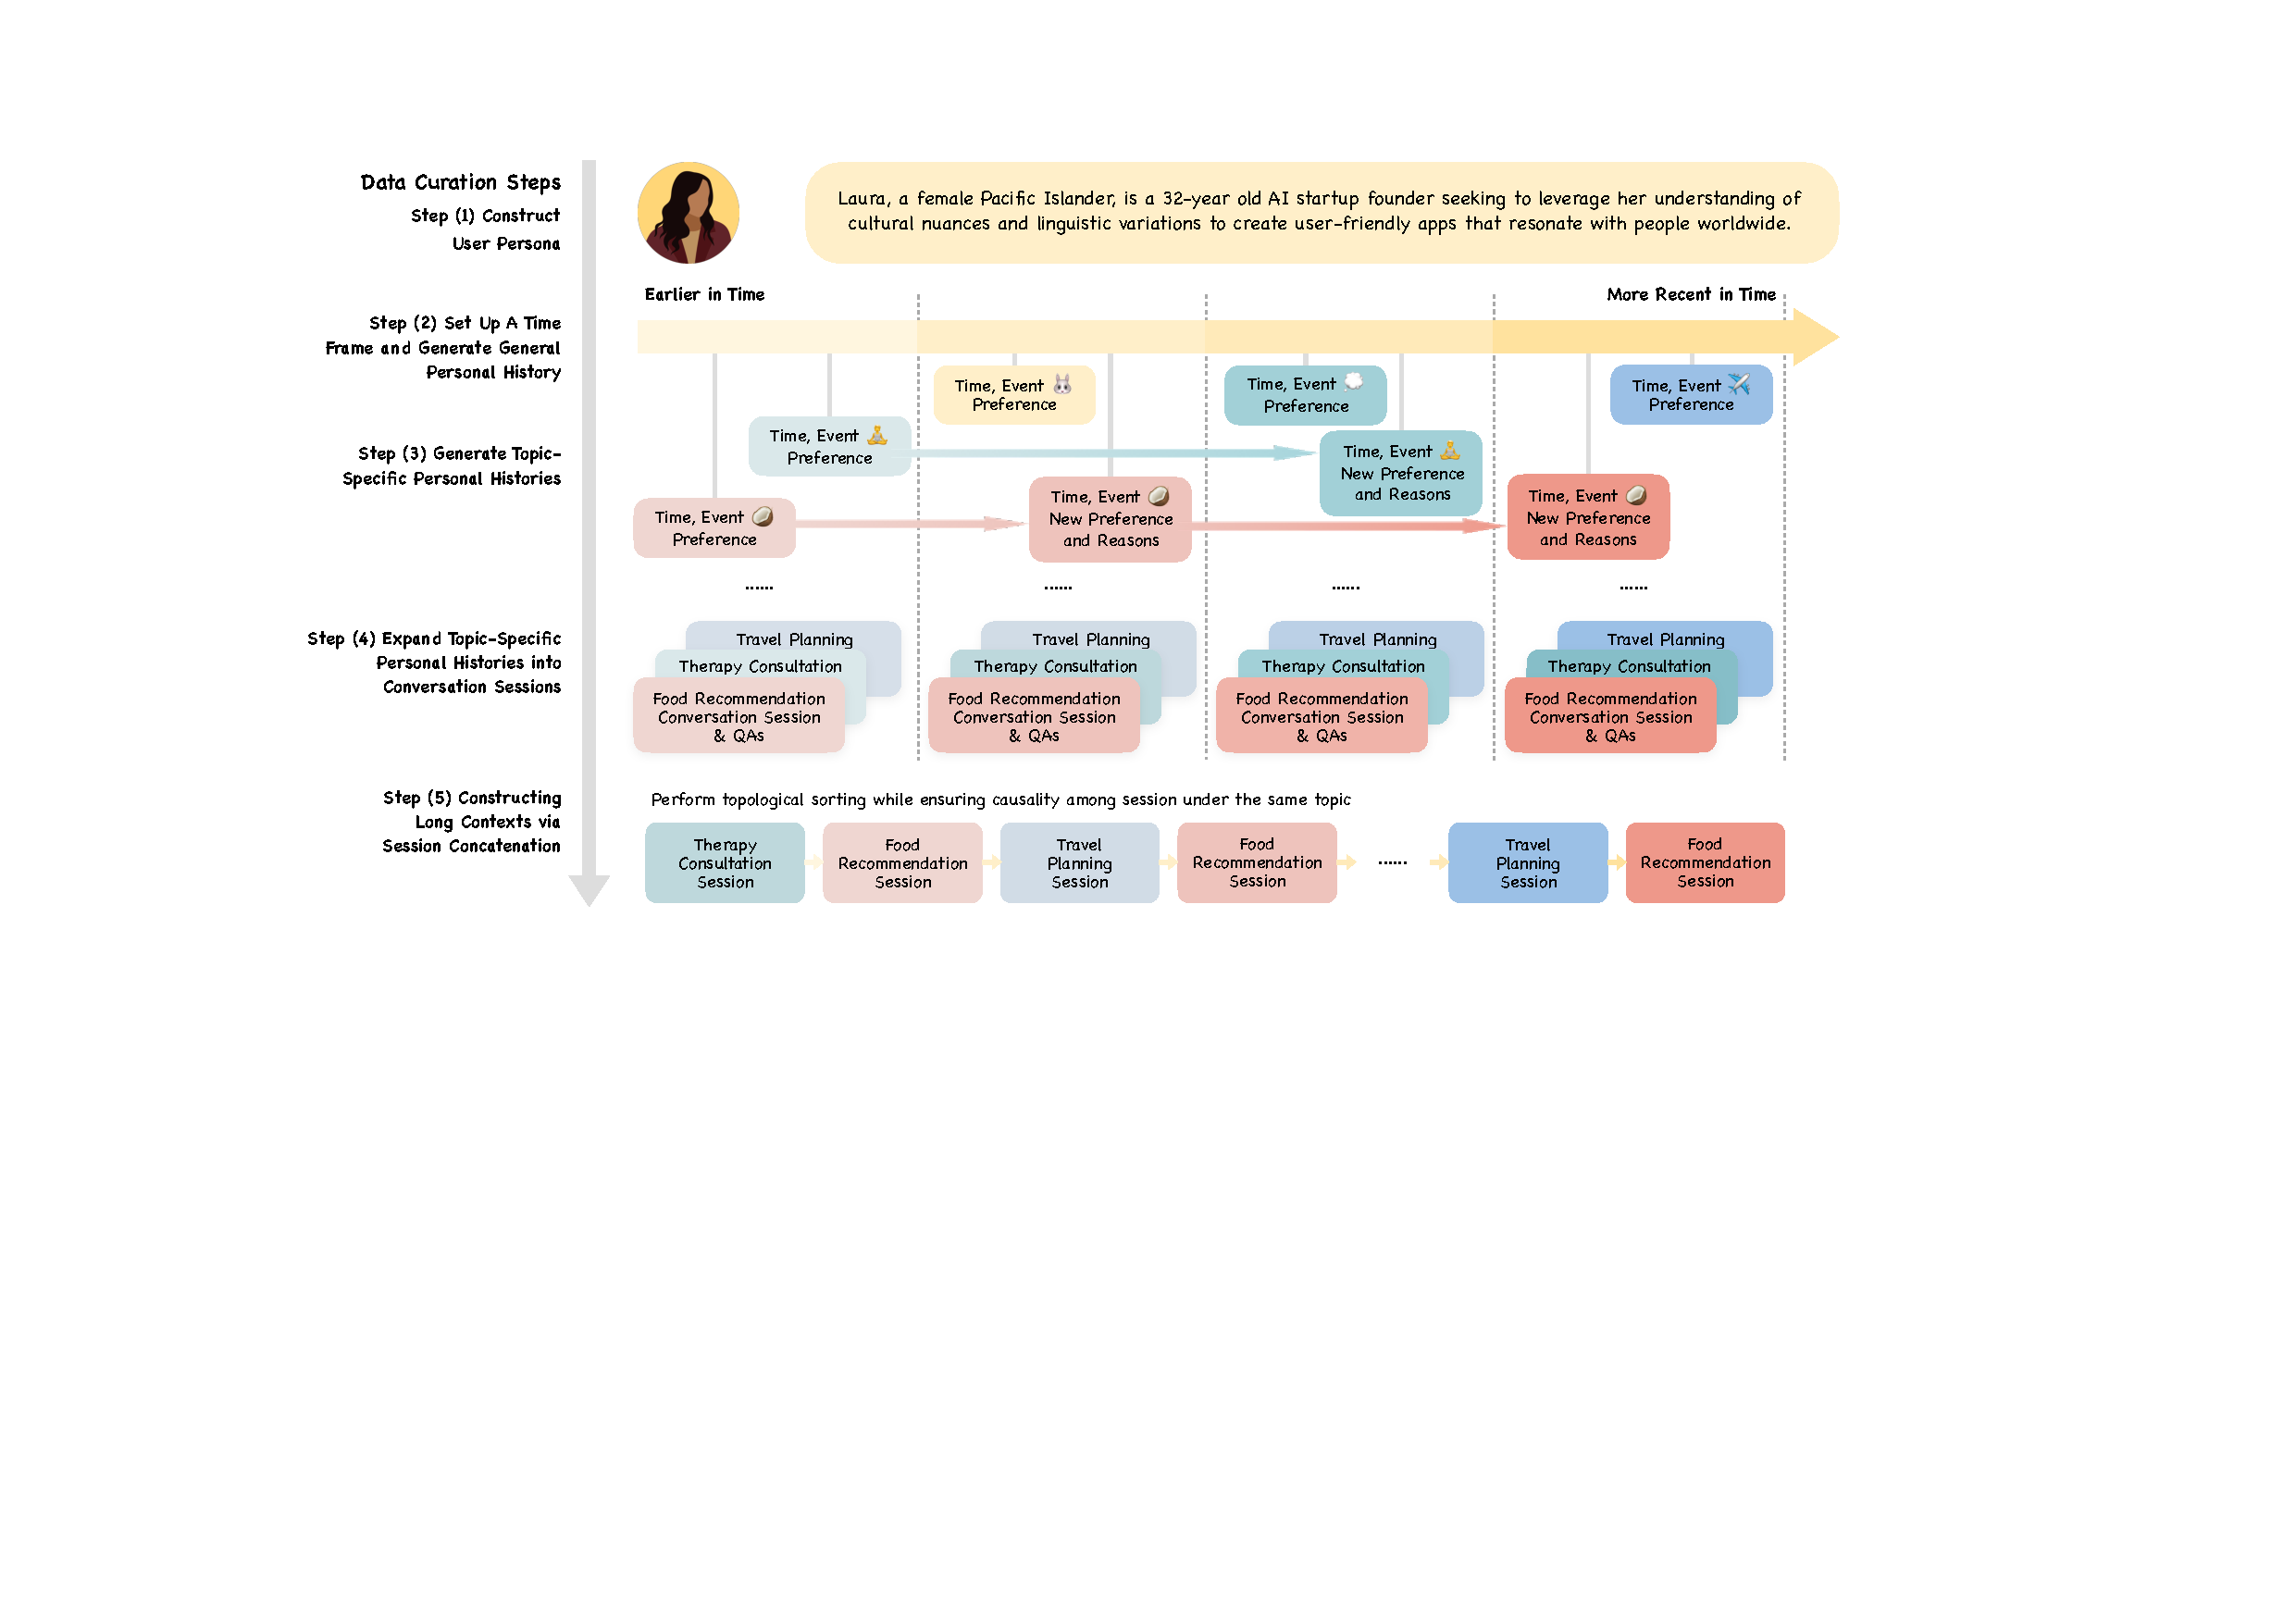
\includegraphics[width=1\linewidth]{figures/generate_data.pdf}
  \caption{\textbf{An overview of the persona-oriented multi-session data curation process}. We construct user personas, build time-stamped general and topic-specific personal histories, expand them into conversation sessions, and topologically concatenate sessions to create long conversation contexts—resulting in a scalable generation framework.}
  \vspace{-2mm}
  \label{fig:generate_data}
\end{figure}

\paragraph{Assemble interaction history via session concatenation.}
Generating large-scale, persona-oriented long-context conversations can be both \textit{cost-efficient} and \textit{scalable}. For each persona, we topologically sort conversation sessions based on their ending timestamps, and we only need to make sure sessions within the same topic maintain causality. \textit{Different numbers of sessions can be concatenated in multiple valid orders.} This flexible design allows for multiple valid interleavings of sessions across different topics, meaning \textit{we only need to generate sessions themselves—not every entire long-context conversation from scratch.} To further extend context length and simulate more natural interactions, we insert a limited number of short interactions between sessions where the user asks random knowledge questions or programming helps without indicating any user preferences.

% \subsection{Resolving the Chicken-and-Egg Dilemma}
% While we leverage GPT-4o to generate conversation data, we also evaluate language models on this generated data. This creates a potential chicken-and-egg dilemma. However, we assume that generating individual conversation sessions—especially with access to structured personal histories—is trivial. In contrast, evaluating model performance over the full, concatenated long-context conversations remains challenging.


% We aim to generate long-context conversation data extending up to one million tokens, significantly surpassing a single conversation session. To achieve this, we need a cost-effective approach for producing numerous long-context samples. Given that we have independently collected one to four conversation sessions per topic — aside from shared persona and general personal history — we can create diverse long-context samples by selecting different subsets of these sessions from multiple topics, arrange them topologically based on their ending timestamps, and concatenate them in different configurations. 

% This approach offers flexibility in constructing long-context conversations. We can concatenate any number of available sessions, and there are multiple valid ways to perform topological sorting on these sessions. Instead of generating each long-context sample from scratch, we can efficiently create multiple versions using only the existing sessions we have already generated, without making additional API calls to any large language models.

% TODO: Add explanation on the chicken-and-egg problems here


% \subsection{Curating of Question-Answering Pairs}
% We implement a multiple-choice question answering framework to evaluate the discriminative setting as mentioned in Section \ref{sec:overview}. This methodology assesses two critical aspects of model performance: comprehension of user personas and tracking of conversational evolution. During the conversation, we simulate the questions users might ask language model agents. Each evaluation item presents both correct answers and strategically designed incorrect options. These incorrect options fall into two categories: factually inaccurate statements and information not present in the conversation history.

% For user-specific recommendation problems, we construct misleading options by modifying correct responses to align with stereotypical characteristics based on general user identities while contradicting specific preferences revealed during conversations. This approach evaluates a crucial capability: the model's ability to differentiate between contextual, user-specific memory and its pre-existing parametric knowledge. Such discrimination is fundamental for effective personalized memorization.

%\subsection{Curation of Generating Personalized Conversation}
%TODO: discuss the metric and implementation for generative settings -- or should we talk about it in experiment section?

% \subsection{Curation of Persona and Event-Grounded Question and Answers}

% TODO

\paragraph{Human validation on dataset quality.}
To evaluate the quality of our generated data, we conduct a human study on 90 random query–response pairs from \datasetname, each grounded in user persona, personal histories, and associated utterances in conversation. Three annotators assess each Q\&A pair across four dimensions: appropriateness, relevance, correctness, and best response. Judgments were very high for all dimensions -- 97.8\%, 95.6\%, 97.8\%, and 90.0\% respectively. Further details are provided in Appendix~\ref{sec:human_eval}.
% To check the quality of our generated data, we perform a human evaluation on a subset of data from \datasetname. As the dataset curation process is complex, we task humans with annotating the final stage -- the questions and answers, paired with the session and metadata they are grounded in. We ask three annotators to binarily evaluate 90 entries on 4 dimensions: appropriateness, relevance, correctness, and best response. We find that the annotators rate all dimensions highly (TODO), and that agreement between them is also high (TODO). Further details are provided in Appendix~\ref{sec:human_eval}.